% compile with: lualatex -shell-escape filename.tex
\documentclass[tikz]{standalone}
\directlua{luatexbase.add_to_callback(
  "wrapup_run",
  function() os.execute("pdf2svg \jobname.pdf \jobname.svg") print("Converted to SVG.") end,
  "final callback to convert pdf file")}

\usetikzlibrary{positioning}

\begin{document}

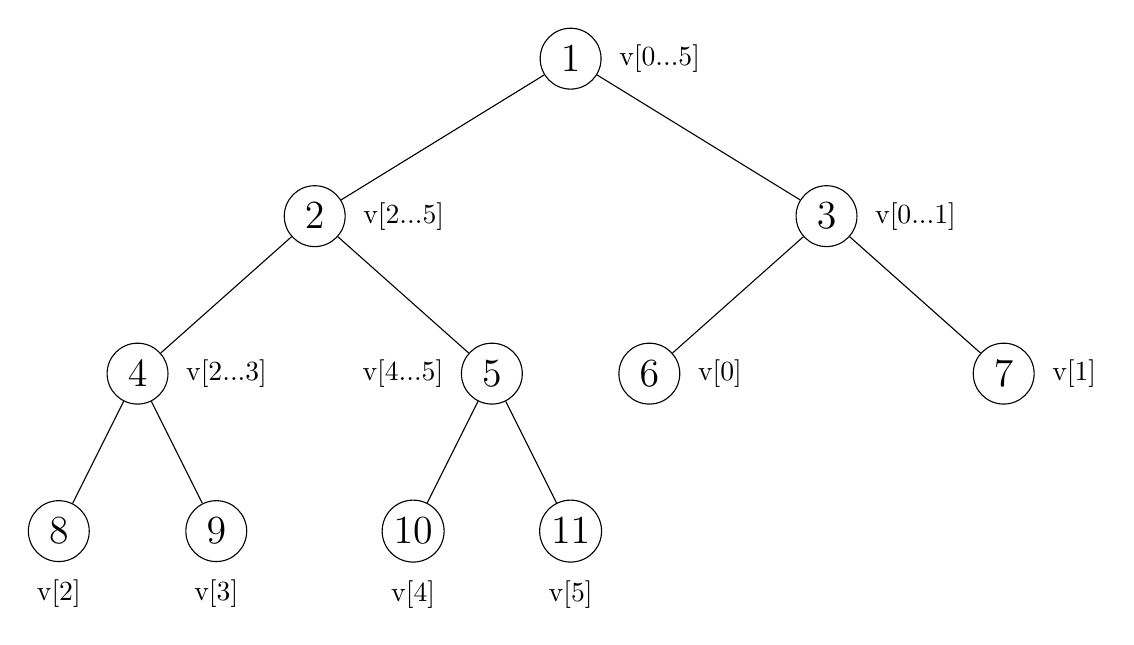
\begin{tikzpicture}[
  tree/.style={
    circle,
    draw,
    font=\Large,
    inner sep=2pt,
    minimum size=22pt,
  },
  level distance=20mm,
  level 1/.style={sibling distance=65mm},
  level 2/.style={sibling distance=45mm},
  level 3/.style={sibling distance=20mm}
  ]
  \node[tree] (n1) {1}
  child {node[tree] (n2) {2}
    child {node[tree] (n4) {4}
      child {node[tree] (n8) {8}}
      child {node[tree] (n9) {9}}
    }
    child {node[tree] (n5) {5}
      child {node[tree] (n10) {10}}
      child {node[tree] (n11) {11}}
    }
  }
  child {node[tree] (n3) {3}
    child {node[tree] (n6) {6}}
    child {node[tree] (n7) {7}}
  };

  \node[right = 1mm of n1] {v[0...5]};
  \node[right = 1mm of n2] {v[2...5]};
  \node[right = 1mm of n3] {v[0...1]};
  \node[right = 1mm of n4] {v[2...3]};
  \node[left = 1mm of n5] {v[4...5]};
  \node[right = 1mm of n6] {v[0]};
  \node[right = 1mm of n7] {v[1]};
  \node[below = 1mm of n8] {v[2]};
  \node[below = 1mm of n9] {v[3]};
  \node[below = 1mm of n10] {v[4]};
  \node[below = 1mm of n11] {v[5]};
\end{tikzpicture}

\end{document}
